\documentclass[11pt]{book}

\usepackage[utf8]{inputenc}   
\usepackage[T1]{fontenc}
\usepackage{lmodern}
\usepackage{geometry}
\geometry{rmargin=3.6cm,lmargin=3.6cm, tmargin=3cm, bmargin=3cm}
\usepackage{courier}
\usepackage{graphicx}
\usepackage{amsmath}
\usepackage{esint}
\usepackage{amssymb}
\usepackage{hyperref}
\hypersetup{
    colorlinks,
    citecolor=black,
    filecolor=black,
    linkcolor=black,
    urlcolor=black
}

\usepackage{amsfonts}
\setlength{\parindent}{0pt}
\begin{document}
\begin{titlepage}
	\centering
	\vspace{1cm}
	{\scshape\LARGE École Polytechnique de Bruxelles \par}
	\vspace{3.5cm}
	{\scshape\Large INFO-F521\par}
	\vspace{.5cm}
	{\huge\bfseries Graphs and Networks\par}
	\vspace{2cm}
	{\Large Martine \textsc{Labbe}, Gwenaël \textsc{Joret}\par}
	\vfill
	Notes by \par
	Charles \textsc{Hamesse}

	\vfill

% Bottom of the page
	{\large \today\par}
\end{titlepage}
\tableofcontents


\chapter{The Basics}
	\section{Graphs}
		A \textit{graph} is a pair $G = (V, E)$ of sets such that $E \subseteq [V]^2$: the elements of $E$ are 2-element subsets of $V$. The elements of $V$ are the \textit{vertices} (or \textit{nodes}, or \textit{points}) and the elements of $E$ are the \textit{edges} (or \textit{lines}). \\
		
		The number of vertices of a graph $G$ is its \textit{order}, written as $|G|$. The number of edges is noted $||G||$. \\
		
		Two vertices $x, y$ of $G$ are \textit{adjacent} or \textit{neighbours} if $x y$ is an edge of $G$. Two edges $e \neq f$ are adjacent if they have an end in common. If all the vertices of $G$ are pairwise adjacent, then $G$ is complete. A complete graph on $n$ vertices is a $K^n$ - a $K^3$ is a triangle.\\ 
		
		Let $G = (V, E)$ and $G' = (V', E')$ be two graphs. We call $G$ and $G'$ \textit{isomorphic}, and write $G \simeq G'$, if there exists a bijection $\varphi: V \rightarrow V'$ with $xy \in E \iff \varphi(x) \varphi(y) \in E'$ for all $x, y \in V$. Such a map $\varphi$ is called an \textit{isomorphism}; if $G = G'$, it is called an \textit{automorphism}. \\
		
		We set $G \cup G' := (V \cup V', E \cup E')$, the intersection is defined similarly with $\cap$. If $G \cap G' = \emptyset$, then $G$ and $G'$ are \textit{disjoint}. If $V' \subseteq V$ and $E' \subseteq E$, then $G'$ is a \textit{subgraph} of $G$ and $G$ is a supergraph of $G'$.\\
		
		If $G' \subseteq G$ and $G'$ contains all the edges $xy \in E$ with $x, y \in V'$, then $G'$ is an \textit{induced subgraph} of $G$; we say that $V'$ \textit{induces} or \textit{spans} $G'$ in $G$,
                and write $G[V'] := G'$.\\

		A \textit{spanning subgraph} $G'$ of a graph $G$ is a subgraph that includes all of the vertices of $G$ ($V' = V$).

	\section{The degree of a vertex}
		Let $G = (V, E)$ be a non-empty graph. The set of neighbours of a vertex $v$ in $G$ is denoted $N_G (v)$, or briefly $N(v)$.\\

		The \textit{degree} (or \textit{valency}) $d_G (v) = d(v)$ of a vertex $v$ is the number $|E(v)|$ of edges at $v$; this is equal to the number of neighbours of $v$. A vertex of degree 0 is $isolated$. \\
		
		The number $\delta(G) := \min~ \{~ d(v) ~| ~v \in V ~\}$ is the \textit{minimum degree} of $G$, the number $\Delta(G) := \max ~\{~ d(v) ~|~ v \in V ~\}$ is the \textit{maximum degree}.\\
		
		If all the vertices of $G$ have the same degree $k$, then $G$ is \textit{k-regular}, or simply \textit{regular}. A \textit{3-regular} graph is called \textit{cubic}.\\

                A \textit{k-factor} is a k-regular spanning subgraph.

	\section{Paths and cycles}
		A \textit{path} is a non-empty graph $P = (V, E)$ of the form:
		\begin{eqnarray*}
			V = \{x_0, x_1, \dotsb, x_k \} ~~~~~~ E = \{x_0x_1, x_1x_2, \dotsb, x_{k-1}x_k\},
		\end{eqnarray*}		
		where the $x_i$ are all distinct. The vertices $x_0$ and $x_k$ are \textit{linked} by $P$ and are called its \textit{endvertices} or \textit{ends}. The other vertices are called the \textit{innervertices}.\\
		
		For $P$ a path from $x_0$ to $x_k$, we write with $0 \leq i \leq j \leq k$:
		\begin{eqnarray*}
			Px_i &:=& x_0 ... x_i\\
			x_iP &:=& x_i ... x_k\\
			x_iPx_j &:=& x_i ... x_j
		\end{eqnarray*}
	
	\section{Connectivity}
	A non-empty graph $G$ is called \textit{connected} if any two vertices are linked by a path in $G$. If $U \subseteq V(G)$ and $G[U]$ is connected, we also call $U$ itself connected in $G$.\\

        \textit{Disconnected} = not connected.\\

		A graph $G$ is \textit{k-connected} (for $k \in \mathbb{N}$) if $|G| > k$ and $G - X$ is connected for every set $X \subseteq V$ with $|X| < k$. In other words, no two vertices of $G$ are separated by fewer than $k$ other vertices.
		
	\section{Bipartite graphs}
		Let $r \geq 2$ be an integer. A graph $G = (V, E)$ is called \textit{r-partite} if $V$ admits a partition into $r$ classes such that every edge has its ends in different classes: vertices in the same partition class must no be adjacent. Instead of "2-partite", one usually says \textit{bipartite}.\\
		
		An $r$-partite graph in which every two vertices from different partition classes are adjacent is called \textit{complete}; the complete $r$-partite graphs for all $r$ together are the \textit{complete multipartite graphs}.



\chapter{Matchings}
Given the graph $G = (V, E)$, the set $M \subseteq E$ is a matching if all edges in $M$ are independent. That is, no two edges share an endpoint. The size of a matching is the number of edges it contains.\\

For the graph $G$, $X \subseteq V$ is a \textit{vertex cover} if every edge in $E$ has at least one endpoint in $X$.\\

A \textit{perfect matching} (a.k.a. 1-factor) is a matching which matches all vertices of the graph. That is, every vertex of the graph is incident to exactly one edge of the matching. Every perfect matching is maximum and hence maximal. In some literature, the term complete matching is used. A perfect matching is also a minimum-size edge cover. \\

Observation: if $M$ is a matching and $X$ a vertex cover, then $|X| \geq |M|$. Corollary: the minimum size of a vertex cover is $\geq$ the maximum size of a matching.

\section{Matching in bipartite graphs}
For this whole section, we let $G = (V, E)$ be a fixed bipartite graph with bipartition $\{A, B \}$. Vertices denoted as $a, a'$, etc will be assumed to lie in $A$, vertices noted as $b$ etc will lie in $B$.\\

An \textit{alternating path} (w.r.t. some matching $M$) is a path in $G$ that starts at an unmatched vertex in $A$ and alternates between edges in $E-M$ and edges in $M$ (it can be made of only one edge).\\

An \textit{augmenting path} (w.r.t. some matching $M$) is an alternating path whose end will be at an unmatched vertex. Note that if $P$ is an augmenting path, then $M \Delta E(P)$ \footnote{$\Delta$, a symmetric difference, defined as $X \Delta Y = (X-Y) \cup (Y-X)$} is again a matching, of size $|M| + 1$. \\

Alternating paths play an important role in the practical search for large matchings. In fact, if we start with any matching and keep applying augmenting paths until no further such improvement is possible, the matching obtained will always be an optimal one, a matching with the largest possible number of edges.

\subsubsection{König's theorem (1931)} 

\textit{The maximum cardinality of a matching in $G$ is equal to the minimum cardinality of a vertex cover.}\\

Let $G = (V,E)$ be a bipartite graph with bipartition $V = (A, B)$. Then the maximum size of a matching in $G$ is the minimum size of a vertex cover in $G$.
	\begin{enumerate}
		\item Let $M$ be a maximum matching. From every edge in $M$ let us choose one of its ends: its end in $B$ if some alternating path ends in that vertex, and its end in $A$ otherwise. We shall prove that this set of these $|M|$ vertices - let us name it $U$ - covers $E$; since any vertex cover of $E$ must cover $M$, there can be none with fewer than $|M|$ vertices, and so the theorem will follow.
		\item Let $ab \in E$ be an edge; we show that either $a$ or $b$ lies in $U$. If $ab \in M$, this holds by definition of $U$ - so we assume that $ab \notin M$. Since $M$ is a maximal matching, there is an edge $a'b' \in M$ with $a = a'$ or $b = b'$ For all $ab \notin M$, we have:
			\begin{enumerate} 
				\item First, let's assume $b = b'$: $a$ is the unmatched start of $ab$, which is then an alternating path, and so the end of $a'b' \in M$ chosen for $U$ was the vertex $b' = b$.
				\item Now with $a' = a$. If the start $a = a'$  is not in $U$, then $b' \in U$ (as $a'b'$ is an edge in $M$), and some alternating path $P$ ends in $b'$ (by definition of $U$). But then there is also an alternating path $P'$ ending in $b$, either $P := Pb$ (if $b \in P$) or $P' := Pb'a'b$. By the maximality of $M$, however, $P'$ can't be an augmenting path. So $b$ must be matched, and was chosen for $U$ from the edge of $M$ containing it.
			\end{enumerate}
	\end{enumerate}
	
\subsubsection{Hall's theorem (1935)} 

\textit{If $G$ is bipartite with partitions $A,B$, it contains a matching of $A$ if and only if $|N(S) \geq |S|$ for all $S \subseteq A$).}\\

Here, $N(S) = \{ x \in B $ s.t. $x$ is adjacent to some vertex in $S \}$.\\

\begin{figure}[h]
	\center
	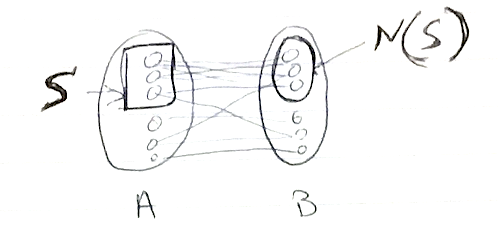
\includegraphics[width=0.3\linewidth]{img/2-1.png}
\end{figure}  
Let $G = (V, E)$ be a bipartite graph with bipartition $V = (A, B)$. Then (keeping in mind that for each partition $X$, any $x \in X$ isn't connected to any other $x' \in X$):
\begin{eqnarray}
	A \text{ can be matched } \iff |N(S)| \geq |S| ~~\forall S \subseteq A
\end{eqnarray} 
Proving both implications:
\begin{enumerate}
	\item $\implies$: done orally, quite intuitive.
	\item $\impliedby$: we prove the contrapositive\footnote{The contrapositive of a statement has its antecedent and consequent inverted and flipped: the contrapositive of $P \rightarrow Q$ is thus $\neg Q \rightarrow \neg P$}: if $A$ cannot be matched then $\exists S \subseteq A$ such that $|N(S) < |S|$. So assume $A$ cannot be matched:
		\begin{eqnarray}
			A \text{ can be matched } &\impliedby& |N(S)| \geq |S| ~~\forall S \subseteq A \\
		\end{eqnarray}
		is equivalent to:
		\begin{eqnarray}
			A \text{ cannot be matched } &\implies& \exists S \subseteq A : N(S) < |S|
		\end{eqnarray} 
	\item If $G$ contains no matching of $A$, then by König's theorem, it has a cover $U$ with fewer than $A$ vertices:
		\begin{eqnarray}
			|A \cap U| + |B \cap U| < |A|
		\end{eqnarray}
		hence:
		\begin{eqnarray}
			|B \cap U| < |A| - |A \cap U| = |A \setminus (A \cap U)|
		\end{eqnarray}
	\item By defintion of $U$, $G$ has no edge between $A \setminus (A \cap U)$ and $B \setminus (B \cap U)$. Let $A \setminus (A \cap U)$:
		\begin{eqnarray}
			|N(S)| \leq |B \cap U| < |A \setminus (A \cap U)| = |S|
		\end{eqnarray} 
		and the marriage condition fails.
\end{enumerate}

	\section{Matching in general graphs}
		Given a graph $G$, let us denote by $\mathcal{C}_G$ the set of its components, and by $q(G)$ the number of its odd components, those of odd order.\\
		
		A \textit{spanning subgraph} $H$ of a graph $G$ is a graph that includes all of the vertices of $G$. 


		\subsubsection{Tutte's theorem (1947)} 
		
		\textit{A graph $G$ has a 1-factor if and only if $q(G - S) \leq |S|$ for all $S \subseteq V(G)$.}\\
		
		Note that a 1-factor corresponds to a perfect matching. Obviously, every odd component of $G - S$ is linked to $S$ by at least one edge from the matching $M$ (because of parity). Hence $|S| \geq q(G - S)$. Let's prove the contrapositive: assume there isn't a perfect matching. We want to show:
			\begin{eqnarray}
				\exists S \subseteq V : |S| < q(G - S)
			\end{eqnarray} 
			A set such as $S$ will then be said "bad".\\
		
		We will make two observations:
		\begin{enumerate}
			\item If $|V|$ is odd, then a set $S = \emptyset$ would be bad because $q(G - S) = q (G)$, then at least one of the components of $G$ must be odd since $|V|$ is odd. Hence $g(G -S) = q(G) \geq 1 > |S| = 0$. So we assume $|V|$ is even.
			\item If $H$ is a graph and $H'$ is a subgraph obtained by deleting some edge $e$ of $H$, then $q(H') \geq q(H)$.
		\end{enumerate}

		\paragraph{Corollary 1} If $H'$ is a spanning subgraph of $H$ then  $q(H') \geq q(H)$.
		
		\paragraph{Corollary 2} If $S$ is a bad set for $H$ then $S$ is bad for all spanning subgraphs of $H$.
		
		We have $q(H -S) > |S|$ since $S$ is bad for $H$. Now if $H'$ is a spanning subgraph of $H$, then $H' - S$ is a spanning subgraph of $H -S$ and thus by Cor. 1, $q(H' - S) \geq q(H - S)$, thus $q(H' - S) > |S|$.
		
		\paragraph{Trick} Let $H$ be obtained from $G$ by iteratively adding edges as long as possible, without creating any perfect matching. By previous observation, if we find a bad set $S$ for $H$ then $S$ is also bad for $G$. Hence, we may focus on $H$.
		
		Say that $S \subseteq V$ is nice. That is, if:
		\begin{enumerate}
			\item Every $v \in S$ is connected to all other vertices from $V - \{ v \}$.
			\item All components of $H - S$ are complete subgraphs
		\end{enumerate}
		Observation: if $S \subseteq V$ is nice, then $S$ is bad. In every component, let's cover all but one vertex. For every odd component, connect the vertex we left to $S$. Indeed, if $S$ were not bad, then we could construct a perfect matching in $H$. But we know there isn't a perfect matching so $S$ is bad.\\
		
		So WMA there isn't a nice $S \subseteq V$. We will show that it leads to a contradiction. Let $S := \{ v \in V : v \text{adjacent to all vertices in} V - \{ v \} \}$. $S$ is the set of universal vertices (satisfies condition 1). By definition, $S$ satisfies condition 1 from the definition of nice subsets. Thus $S$ must violate condition 2. That is, there is a component $X$ of $G - S$ which is not complete, i.e. $\exists a, a' \in X$ such that $aa' \notin E$. Consider a shortest path between $a$ and $a'$, and let $a, b, c$ be the first three vertices on that path. Since $b \notin S$, $\exists d \in V$ such that $bd \notin E$. There is a perfect matching $M_1$ in $H + ac$, also there's a perfect matching in $M_2$ in $H + bd$ 
		
		Note: we know there are at least 3 vertices in this component to have a least 1 connection: components are connected.

		\subsubsection{Tutte's proof 2}
			Let $H + ac$ have a perfect matching $M_1$ and $H + bd $ have a perfect matching $M_2$.
			With:
			\begin{eqnarray}
				M_1 \Delta M_2 = (M_1 - M_2) \cup (M_2 - M_1)
			\end{eqnarray}
			We get an "alternating" path of pink / blue edges (which are in the symmetric difference), paths alternating between colours, which goes back to the starting point (i.e. a cycle) because the graph is finite and botch matchings are perfect. Also, there could be as many cycles as we want. \\
			
			Now, using this result: remember that $ac$ is an edge of $M_1$, as $bd$ is in $M_2$, not in the other:
			\begin{eqnarray}
				bd \in M_1 \Delta M_2
			\end{eqnarray}
			Then $bd$ is in a cycle $C$ in $M_1 \Delta M_2$.
			We have several cases:
			\begin{enumerate}
				\item $ac \notin E(C)$: there's a cycle containing $bd$. We can switch $M_2$ on the cycle (i.e. $M_2 \Delta E(C)$: still getting a perfect matching which avoids $ac$ and $bd$, this is a p.m. in $H \longrightarrow $ contradiction.
				\item $ac \in E(C)$: the cycle contains $ac$. We cannot do the switch because we lose $bd$ and $ac$ appears in $M_2$: the new perfect matching... wasn't a perfect matching. The idea is: shortcut $c$ as in $bc$ then we can do the switching and $M_2 \Delta E(C')$ is a p.m. in $H \longrightarrow$ contradiction.
			\end{enumerate}
			


\chapter{Connectivity}
	A (non empty) graph is \textit{connected} when there is a path between every pair of vertices. In a connected graph, there are no unreachable vertices. A graph that is not connected is \textit{disconnected}.\\

	A graph with just one vertex is connected. An edgeless graph with two or more vertices is disconnected.\\
	
	A graph $G$ is \textit{$k$-connected} if $|V(G)| \geq k + 1$ and $\nexists X \subseteq V$ with $|X| \leq k-1$ such that $G-X$ is disconnected.\\
	
	The \textit{vertex connectivity} of $G$ is the maximum $k$ so that $G$ is $k$-connected.\\
	
	A vertex $v \in V(G)$ is a \textit{cut vertex} of a connected graph $G$ is $G - \{ v \}$  is not connected.

	\section{2-Connected graphs and subgraphs}
		There are at least 3 vertices and there isn't any cut vertex.\\
		
		A \textit{block} of a graph $G$ is an induced subgraph $B$ of $G$ such that $B$ is connected and has no cut vertex and $B$ is maximal with this property.\\
		
		A block $B$ can be:
			\begin{itemize}
				\item a \textit{bridge}: $B = \{x,y\}$ with $xy \in E(G)$ and $G - xy$ is disconnected.
				\item a 2-connected induced subgraph: if $|B| \geq 3$, and $B$ is maximal with this property.
				\item a single vertex: $|B| = 1$, when $G$ has a singleton component.
			\end{itemize}
			
		Let us make an observation: if $B_1$ and $B_2$ are two distinct blocks, then they have at most one vertex in common, and if they do then that vertex is a cut vertex of $G$.\\
		
		And another: let's make a bipartite graph with, on the one hand, the blocks and on the other hand, the cut vertices.\\

                Blocks define a tree structure (no cycle).

		\subsection{Theorem: ear decomposition of 2-connected graphs}
		Let $G$ be 2-connected $\iff G$ can be built starting with a cycle and iteratively adding ears.\\
		
		Proof: 
		\begin{enumerate}
			\item $\impliedby$ OK
			\item $\implies$ Let $H \subseteq G$ be a subgraph of $G$ that can be constructed by the procedure and maximal with this property. Note that $H$ exists because $G$ has at least one subgraph that can be constructed, namely a cycle (since $G$ is 2-connected). We want to show $H = G$. Suppose not (pf by contradiction): 
				\begin{enumerate} 
					\item $V(H) = V(G) \implies \exists e \in E(G) - E(H)$ then we could have added $e$ to $H$, contradicting the maximality of $H$.
					\item $V(H) \neq V(G)$. We connect a vertex from an ear to a vertex from the cycle $H$. Since $G$ is connected, $\exists ab \in E(G)$ with $a \in V(H), b \notin V(H)$. Since $G$ is 2-connected, $G-a$ is connected, so there is a path $P$ linking $b$ to $V(H) - \{a\}$ in $G- a$, hence we could have added the ear $P + ab$ to $H \rightarrow$ contradiction. 
				\end{enumerate}
		\end{enumerate}
		
		
	\section{The structure of 3-connected graphs}
		\subsection{Lemma (Tutte)}
		\textit{If $G$ is 3-connected and $|V(G)| \geq 5$, then $\exists e \in E (G)$ such that $G / e$ is still 3-connected.}\\
		
		Note that $G / e$ is the graph $G$ following the contraction of the edge $e$.\\
		
		Proof: by contradiction, assume there is no such edge.
		\begin{enumerate}
			\item Consider any edge $xy \in E(G)$. Now $H := G / xy$ is not 3-connected, thus there is a subset $S$ of vertices of $H$ with $|S| \leq 2$ so that $H - S$ is not connected. 
			\item Observation: if $v_{xy}$ denotes the vertex of $H$ resulting from the contraction of $xy$, then we must have $v_{xy} \in S$, because without otherwise $S$ would also be a cut set of $G$ of size $\leq 2$.
			\item On the  other hand, if $S'$ is obtained from $S$ by replacing $v_{xy}$ with $x,y$ then $S'$ is a cut set of $G \implies |S'| \geq 3 \implies |S| = 2$.
		\end{enumerate}
		
		Any 3-connected graph can be contracted to $K_4$ by iteratively contracting edges, in such a way that each intermediate state remains 3-connected.
		
		
	\section{Menger's theorem}
		\textit{Let $G = (V,E)$ be a graph and $A, B \subseteq V$. Then the minimum number of vertices separating $A$ from $B$ in $G$ is equal to the maximum number of disjoint $A-B$ paths in $G$.\\}

		\begin{enumerate}
			\item Proof $\impliedby$: Take distinct $a ,b \in V(G)$. Since there are $k$ independent $a-b$ paths and at least $k-1$ of these have at least one internal vertex, $G$ has $\geq 2 + k - 1 = k + 1$ vertices. Moreover, there is no $Y \subseteq V(G)$ of size less than $k$ such that $G - Y$ is not connected, because o/w: pick $a,b$ in distinct components of $G - Y$. Every $a-b$ path goes through $Y$, hence there cannot be $k$ independent $a-b$ paths.
			\item Proof $\implies$: consider two distinct vertices $a,b \in V(G)$. 
		\begin{enumerate}
		\item{Case 1: $ab \notin E(G)$}
		Let $A := N(a)$ and $B := N(b)$.
		If there are $k$ disjoint $A-B$ paths then there are $k$ such paths avoiding $a,b$ and we see that there are $k$ independent paths in $G$.  Observe $|A| \geq k$ and $|B| \geq k$.\\
		
		If $\not{\exists} k$ disjoint $A-B$ paths then $\exists A-B$ separation $Y$ of size $< k$ but this contradicts the fact that $G$ is $k$-connected.
		
		\item{Case 2: $ab \in E(G)$}
		Let $A := N(a) - \{b\}$ and $B := N(b) - \{a\}$. Then $|A| \geq k -1$ and $|B| \geq k - 1$. As always when we have an edge that's annoying, we try to contract it or to delete it:  consider  $G - ab$. This graph is $(k-1)$-connected (this always stands for $k$-connected graphs). And we can find $(k-1)$ disjoint $A-B$ paths in $G - ab$ avoiding $a,b$. So adding $a,b$ and using the edge $ab$ we get $k$ independent $a-b$ paths in $G$. 
		\end{enumerate} 
		\end{enumerate}


\subsection{Menger's theorem (global version)}
$G$ is $k$-connected $\iff$ every pair $a,b$ of distinct vertices are linked by $k$ independent paths (no vertex in common except for $a$ and $b$).


\chapter{Planar graphs}
		A \textit{plane graph} is a pair $G = (V,E)$ where $V \subseteq \mathbb{R}^2$ such that:
		\begin{enumerate}
			\item Every edge is an arc linking two distinct vertices
			\item $\forall e \in E$, the interior $\text{int}(e)$ (the arc, minus the two vertices) contains no vertex of $G$ nor any point from edges $f \in E \setminus \{ e \}$.
			\item Every pair of vertices is linked by at most one edge.
		\end{enumerate}
		Without the third condition, this could be a plane multi-graph (possibly involving "parallel" edges).\\
		
		A plane graph defines a corresponding abstract graph $G$. With a slight abuse of notation, we will write $G$ both for the abstract graph and for the corresponding subset of the plane: $V \cup \Large{\cup_{e \in E}} e \subseteq \mathbb{R}^2$.\\
		
		The \textit{faces} of $G$ are the regions of $\mathbb{R}^2 \setminus G$. Exactly one of these faces is unbounded and is called the \textit{outer face}. The other faces are called \textit{inner faces}. \\
		
		All acyclic plane graphs will have only an outer face. As soon as there is a cycle, there will be at least one inner face. In other words: a plane graph has only one face (the outer face) $\iff$ it is a forest. 
		
		\subsection{Lemma 1} 
		\textit{Let $F \in E(G)$. Then:}
		\begin{enumerate}
			\item $\partial F \subseteq G$
			\item \textit{$\forall e \in E(G)$, either $e \in \partial F$, or $\partial F \cap \text{int}(e) = \emptyset$}
			\item \textit{If $e \in E(G)$ is on a cycle $C \in G$, then $e$ is contained in the boundary of exactly two faces of $G$, one inside $C$ and the other outside $C$.}
			\item \textit{If $e \in E(G)$ is not included in any cycle, then $e$ appears in the boundary of exactly one face.}
		\end{enumerate}
		
		
		\subsection{Lemma 2}
		\textit{If $G$ is a 2-connected plane graph, then the boundary of every face is a cycle of $G$.\\}
		
		Some other properties:
		\begin{itemize}
			\item A graph is planar if it can be realised as a plane graph.
			\item A plane graph is \textit{maximally plane} if one cannot add any edge to it (while staying a plane graph).
			\item A plane graph is a \textit{plane triangulation} if every face is bounded by a triangle of the graph.
		\end{itemize}
		
		
		\subsection{Lemma 3}
		\textit{A plane graph on at least 3 vertices is maximally plane $\iff$ it is a plane triangulation}
		
		
		\subsection{Theorem 1: Euler's formula}
		\textit{Let $G$ be a connected plane graph with $n$ vertices, $m$ edges and $f$ faces. Then:}
		\begin{eqnarray}
			n - m + f = 2
		\end{eqnarray}
		\textit{Note that this formula works only for connected graphs.\\}
		
		Let's prove it with induction on $m$.
		\begin{enumerate}
			\item Base case: $m = n -1$ (as it's connected, it contains a spanning tree, it has $n - 1$ edges). In this case $G$ is a tree and $f = 1$. So $n - m + f = 2$.
			\item Inductive step: $m \geq n$. The connected graph is not a tree, then it has a cycle. Consider a cycle of $G$ and let $e \in E(C)$. The edge is on the cycle, so it's on the boundary of exactly two distinct faces of the graph $F_1, F_2 \in F(G)$. If we remove this edge from the graph, the graph stays connected but two faces merge so $f$ decreases by 1. So $f \rightarrow f -1$, $m \rightarrow m - 1$ and $n$ remains the same. Then $-m + f$ is constant and $n -m + f = 2$.
		\end{enumerate}
		
		\subsection{Corollary 1} 
		\textit{If $G$ is an $n$-vertex plane graph with $n$ being at least $3$, then $G$ has at most $3n - 6$ edges.\\}
		
		With my assumption WLOG that $G$ is maximally plane, i.e. $G$ is a plane triangulation. Let $m := |E(G)|$ and $f := |F(G)|$.
		\begin{eqnarray}
			3f = \sum_{F \in F(G)} 3 = 2m
		\end{eqnarray}
		If we look at every face in the triangulation, each edge will be counted two times as it is boundary to two faces. Hence:
		\begin{eqnarray}
			m = \frac{3}{2} f
		\end{eqnarray}
		And by Euler's formula (which we will use as we're considering a plane triangulation):
		\begin{eqnarray}
			n - m + f = 2
		\end{eqnarray}
		Thus 
		\begin{eqnarray}
			n - m + \frac{2}{3}m &=& 2 \\
			\implies n - \frac{1}{3} m &=& 2 \\
			\implies m &=& 3n - 6
		\end{eqnarray}
		
		\subsection{Corollary 2}
		\textit{$K_5$ is not planar.\\}
		
		$K_5$ has $n = 5$ vertices and $m = 10$ edges but $3n - 6 = 9 < 10$.
		
		
		\subsection{Lemma 3}
		\textit{If $G$ is an $n$-vertex plane graph ($n \geq 3)$ and has no triangle (i.e cycle of length 3 or 3 vertices that are pairwise adjacent), then $G$ has at most $2n - 4$ edges.\\}
		
		\subsection{Corollary 3}
		\textit{$K_{3,3}$ is not planar.\\}
		
		$K_{3,3}$ has $n = 6$ vertices and $m = 9$ edges: $2n - 4 = 8 < 9$.
		
		\subsection{Corollary 4}
		\textit{No planar graph contains $K_5$ or $K_{3,3}$ as a minor.}
		
		\subsection{Theorem 2: Kuratowski (1930)}
		\textit{A graph $G$ is planar $\iff$ $G$ it has neither $K_5$ nor $K_{3,3}$ as minor.\\}
		
		\begin{enumerate}
			\item $\implies$: already done.
			\item $\impliedby$: We first prove the statement in the case that $G$ is 3-connected. That is, we will show: "$G$ 3-connected and has neither $K_5$ or $K_{3,3}$ as minor $\implies$ $G$ is planar", by reduction on $|V(G)|$.
				\begin{enumerate}
					\item Base case: $|V(G)| = 4$. Then $G = K_4$ and is planar (every $k$-connected graph has at least $k+1$ vertices).
					\item Inductive step: $|V(G)| \geq 5$. By Tutte's theorem, there is an edge $xy \in E(G)$ such that when we contract (we get $G \setminus xy$), the graph is 3-connected. Note that $G \setminus xy$ has no $K_5$ nor $K_{3,3}$ minor (by transitivity of the minor relation), thus $G \setminus xy$ is planar by induction. Let $v_{xy}$ be the vertex resulting from the edge contraction. Consider a drawing of $G \setminus xy$ in the plane. The plane graph $(G \setminus xy) - v_{xy}$ is 2-connected. In particular, each face is bounded by a cycle of that graph. Let $C$ denote the cycle bounding the face where $v_{xy}$ was drawn.
\begin{figure}[h]
	\center
	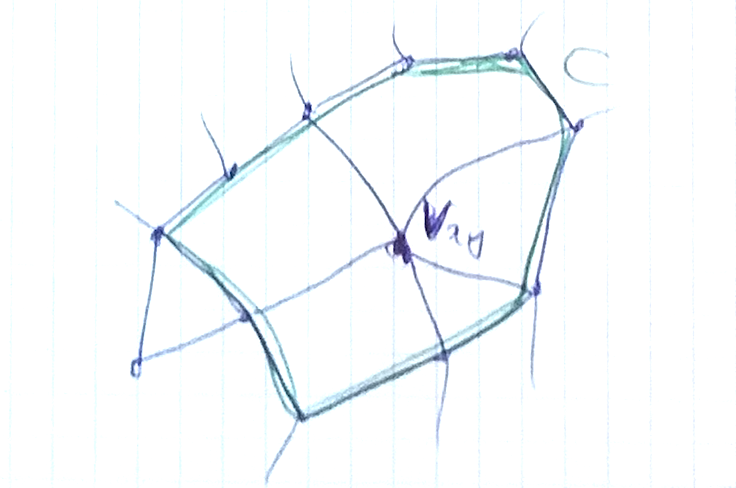
\includegraphics[width=0.3\linewidth]{img/4-1.png}
\end{figure}

Then all neighbours of $v_{xy}$ in $G \setminus xy$ are on $C$. Let:
						\begin{eqnarray}
							X &:=& \{ v \in V(C) : vx \in E(G)\}\\
							Y &:=& \{ v \in V(C) : vy \in E(G) \}
						\end{eqnarray}
						Note that $|X| \geq 2$ and $|Y| \geq 2$, since $G$ is 3-connected.\\
						\begin{figure}[h]
	\center
	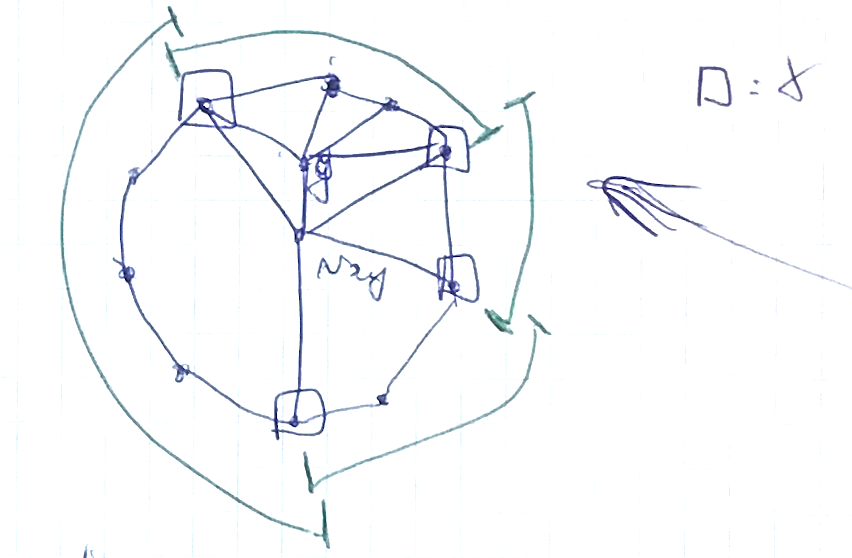
\includegraphics[width=0.3\linewidth]{img/4-2.png}
\end{figure}

Consider the plane graph $H := (G \setminus xy) - \{ vy : v \in Y -X \}$. Note that all the remaining edges are at least adjacent to $X$.
						\begin{enumerate}
							\item Vertices of $X$ define intervals of $C$. One can see $H$ as a plane drawing of $G - y$ (where $v_{xy}$ plays the role of $x$). Our aim is to add $y$ to obtain a drawing of $G$.
							\item If there exists a single interval containing all of $Y$ then we can extend this drawing to a drawing  of $G$ by adding $y$ in the face made by the vertices of $Y$.
							\item Now let's assume this is not the case. We will show that this leads to a contradiction (and this $Y$ must be contained in a single interval).
								\begin{enumerate}
									\item $|X \cap Y| \geq 3$, then there is a $K_5$ minor in $G$.
									\begin{figure}[h]
	\center
	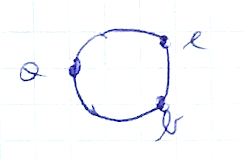
\includegraphics[width=0.3\linewidth]{img/4-3.png}
\end{figure}

Let $a,b,c \in X \cap Y$ be distinct. Consider the minor of $G$ obtained by contracting each of these three paths into edges.
			
			Then in that minor $\{ a,b,c,x,y \}$ are pairwise linked ($a,b,c$ are a triangle, $x$ and $y$ are both connected to all $a,b,c$). Hence $K_5$ is a minor of $G$. Contradiction.
									


									\item $|X \cap Y| \leq 2$, then there is a $K_{3,3}$ minor in $G$: 
									\begin{figure}[h]
	\center
	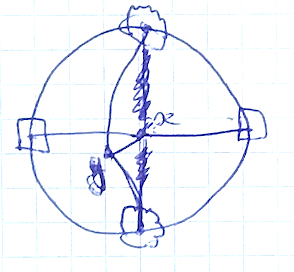
\includegraphics[width=0.3\linewidth]{img/4-4.png}
\end{figure}
								\end{enumerate}
						\end{enumerate} 
				\end{enumerate}
		\end{enumerate}
		
		\textit{Note this usual approach in graph theory: assume the graph has some connectivity, prove the theorem, then extend}
		


\chapter{Colouring}
A vertex colouring of a graph $G = (V,E)$ is a map $\phi: V \rightarrow S$ such that $\phi(u) \neq \phi(v) ~~\forall uv \in E(G)$.

$S$, set of colours. Implicitly $\subset \mathbb{N}$.

\bigskip
If $\phi$ is a $k-$coloring, $|S| \leq k$. Also, we define the \textit{chromatic number} $\chi$ as:
\begin{eqnarray}
	\chi (G) := \min \{ k : \exists k\text{-colouring of }G \}
\end{eqnarray}

A graph $G$ with $\chi_{G} = k$ is called $k-$chromatic; if $\chi_{G} \leq k$, we call $G$ $k-$colourable.\\

Note that $k-$colouring is nothing but a vertex parition into $k$ independent sets, now called \textit{colour classes}. The non-trivial 2-colourable graphs, for example, are precisely the bipartite graphs.

	\section{Colouring maps and planar graphs}
		\subsection{The four colour conjecture (1852)}
		\textit{If a graph $G$ is planar, then $\chi_{G} \leq 4$.	\\}
		
		The has been "proved" by Appel and Haken in 1977 using 2000 graph configurations (resulting in 200 pages). but none has really accepted their proof. \\
		
		Then it has been reproved by Robertson, Saners, Seymour, Thomas (1997, 600 configurations, 160 pages), who tried to understand the first proof but couldn't make sense of it. \\
		
		In 2005, Gonthiers (Microsoft research) made a complete formal proof so that it can be verified by computers, which it has.
		
		\subsection{The five colour theorem (Kempe and Heawood, 1890)}
		\textit{If $G$ is planar, $\chi_{G} \leq 5$.\\}
		
		Proof: by induction on $|V(G)|$, valid if $|V(G)| \leq 5$ so let's assume $|V(G)| \geq 6$. 
		\begin{enumerate}
			\item The average degree of $G$ is:
				\begin{eqnarray}
					d(G) = \frac{\sum_{v \in V(G)} d(v)}{|V(G)|} = \frac{2 |E(G)|}{|V(G)|} \leq \frac{2 (3|V(G)| - 6)}{|V(G)|} < 6
				\end{eqnarray}
				Now if this average is strictly less than 6, there is at least one vertex $v$ with $d(v) \leq 5$.

			\item If $d(v) \leq 4$, then consider a 5-colouring of $G-v$, one colour is available at $v$, done.
			\item If $d(v) = 5$, showing that $\chi_{G}$ could be 6 is now quite straightforward, think of removing $v$ and then putting it back in $G$). Now we have a potential problem if we consider a 5-colouring: there must be two distinct non-adjacent vertices $x, y$ in the neighbours of $v$ such that $xy \notin E(G)$. We will first contract $xv$ and $yv$ (thus keeping the planar property, so we can apply induction). By induction, $G / \{ vx, vy \}$ has a 5-colouring $\phi'$. Let:
				\begin{eqnarray}
					\phi(w) &:=& \phi'(w) ~\forall w\ \in V(G) - \{ vx, vy \}\\
					\phi(x) &:=& \phi(v) := \phi(y) = \phi'(\text{contracted vertex})
				\end{eqnarray}
				$\phi$ is not a valid colouring because of the edges $vx, vy$. However, these are the only two problematic edges. Moreover, since $\phi(x) = \phi(y)$, there is some colour $c$ that is not used on any neighbour of $v$, thus setting $\phi(v) := c$ makes $\phi$ a valid 5-colouring.
		\end{enumerate}
		
		
		\subsection{Discharging method (Weinicke, 1904)}
		\textit{One example to prove above's theorem. If $G$ is a plane triangulation and $G$ has minimum degree $5$, then $\exists vw \in E(G)$ such that $d(v) = 5$ and $d(w) \in \{ 5, 6 \}$.\\}
		
		Put a charge of 6-$d(v)$ on each $v \in (G)$ with:
		\begin{eqnarray}
			\sum_{v \in V(G)} \text{charge}(v) &=& 6 |V(G)| - \sum_{v \in V(G)} d(v) = 6 |V(G)| - 2 |E(G)|\\
			&=& 6 |V(G)| - 2 (3|V(G)| - 6) \\
			&=& 12 > 0
		\end{eqnarray}
		As we're in a plane triangulation, we can use Euler's formula.\\
		
		One dicharging rule: every degree-5 vertex sends  a charge of $1/5$ to each of its neighbours.\\
		
		Let \text{charge'}$(v)$ denote the new charge of $v$. 
		\begin{eqnarray}
			\sum_{v \in V(G)} \text{charge'}(v) = \sum_{v \in V(G)} \text{charge}(v) = 12 > 0
		\end{eqnarray}
		Let $v \in V(G)$ be such that charge'$(v) > 0$. Now we need to do a simple case analysis:
		\begin{enumerate}
			\item $d(v) \in \{ 5,  6 \}$. Then $v$ received some charge from some neighbour $w$, which thus has degree 5 and hence $vw$ is an edge as desired.
			\item $d(v) \geq 8$. This cannot happen because:
				\begin{eqnarray}
					\text{charge'}(v) &\leq&  \text{charge}(v) + d(v)/5\\
					&=& 6 - d(v) + d(v)/5\\
					&=& 6 - \frac{4}{5}d(v)\\
					&\leq& 6 - \frac{4 \cdot 8}{5} < 0
				\end{eqnarray}
			\item $d(v) = 7$. By the same calculation, $v$ receives charges from at least 6 from its neighbours. With the condition that the new charge must be strictly positive, we can find two neighbours of $v$ that have degree 5 and are adjacent.
		\end{enumerate}
		
	A \textit{clique} is a set of pairwise adjacent vertices. A clique of size 3 is a triangle. We have:
	\begin{eqnarray}
		w(G)  := \text{maximum size of a clique in }G
	\end{eqnarray}
	Clearly, $\chi(G) \geq w(G) ~\forall G$. For example, a cycle of 5 vertices has a clique of size 2 but requires 3 colours. Formally, we have $\chi(C_{2k + 1}) = 3$ but $w(C_{2k + 1}) = 2$, for $k \geq 2$.\\
	
	In fact, there are triangle-free graphs (i.e. $w \leq 2$) with arbitrarily high $\chi$.\\
	
	The \textit{girth} of a graph $G$ is the length of a shortest cycle contained in $G$. Its value is considered infinite if $G$ has no cycle.
	
		\subsection{Theorem (Erdős, 1950)}
		\begin{eqnarray}
			\forall k \geq 1, \exists G : \chi(G) \geq k \wedge \text{girth}(G) \geq k
		\end{eqnarray}
		
		One can always 2-colour a tree. If locally, up until some extent, the graph is a tree but contains a cycle globally, the cycle will enforce the value of $\chi$.\\
		
		The chromatic number is a global phenomenon.
		
	So the clique size is a lower bound, but at times this can be a very bad bound. For bipartite graphs, we have equality, but that's not always so.
	
	\section{Perfect graphs}
		
		We use the notation:
		\begin{itemize}
			\item $\omega(G) = $ max size of a clique in $G$
			\item $\alpha(G)$ = max size of a stable set (= an independent set) 
		\end{itemize}
		
		Clearly, $\chi(G) \geq \omega(G) ~\forall G$.\\
		
		A graph $G$ is \textit{perfect} if $\chi(H) = \omega(H)$ for all induced subgraphs $H$ of $G$. For example, bipartite graphs are perfect.\\

		

\subsection{Weak perfect graph conjecture}
$G$ perfect $\iff \overline{G}$ perfect.

\subsection{Strong perfect graph conjecture}
$G$ perfect\\
$\iff$ neither $G$ nor $\overline{G}$ contain odd cycle of length at least $5$
as an induced subgraph.

	
	


	\subsubsection{Theorem (Lovász, 1972)}
	\textit{$G$ perfect
$\iff \alpha(H)\,\omega(H) \geq |H|
\qquad\forall$ induced subgraph $H$ of $G$.\\}

\textit{Stability number}
$\alpha(G) :=$ max size of a stable set (independant set).
	
	\begin{enumerate}
		\item $\implies$: if $H$ is an induced subgraph of $G$, then:
			\begin{eqnarray}
				\alpha(H) \geq \frac{|V(H)|}{\alpha(H)} = \frac{|V(H)|}{\omega (H)}
			\end{eqnarray}
			which is true for every graph. Indeed, if $G$ is perfect, then every induced subgraph $H$ of $G$ can be partitioned into at most $\omega(H)$ colour classes, each containing at most $\alpha(H)$ vertices.
		\item $\impliedby$: by induction on $|V(G)|$.
			\begin{itemize}
				\item Base case: $|V(G)| =1$, $G$ is the only induced subgraph:\begin{eqnarray}
					\alpha(H) \omega(H) \geq |V(H)| = 1
				\end{eqnarray} 
				\item Inductive step: we have to show that $\chi(H) = \omega(H) ~\forall$ induced subgraph $H$ of $G$. If $|V(H)| < |V(H)|$, then we already know that $H$ is perfect thanks to induction. So it remains to show $\chi(G) = \omega(G)$, by contradiction: assume $\chi(G) > \omega(G) \iff \chi(G) \geq \omega(G) + 1$.\\
					
					Observe: if $U$ a a stable set, $U \neq \emptyset$, then $\chi(G-U) = \omega(G-U) \leq \omega(G)$. On the other hand, $\chi(G) \leq \chi(G-U) + 1 \leq \omega(G) + 1$. Hence $\chi(G) = \omega(G) + 1$ and $\chi(G-U) = \omega(G-U) = \omega(G)$.\\
					
					Let $A_0 = \{u_1, u_2, ..., u_{\alpha}$ be a stable set of $G$ of size $\alpha(G)$. Let $\alpha = alpha(G)$ and $\omega = \omega(G)$. For each $i \in \{1, ..., \alpha\}$, consider a colouring of $G - U$ with $\chi(G \setminus U_i) = \omega$ colours and let (...?) $A_{(i-1) \omega + 1}, ..., A_{(i-1) \omega + \omega - 1}, A_\omega$ denote the colour classes.\\
					
					For each $j \in \{0,1,..., \omega\}$, let $K_j$ be a clique of $G - K_j$ of size $\omega(G - K_j = \omega(G) = \omega$.\\
					
					Claim: $\forall i,j \in \{0,1,...,\alpha \omega \}$:
					\begin{eqnarray}
						|A_i \cap K_j| = \begin{cases}
							0 ~~~ \text{if } i = j\\
							1 ~~~ \text{if } i \neq j
						\end{cases}
					\end{eqnarray}
					
					Proof: Clearly, $|A_i \cap K_j| = 0$ if $i=j$. Now let's show that  $|A_i \cap K_j| = 0$ implies $i = j$: assume  $|A_i \cap K_j| = 0$.
						\begin{enumerate}
							\item $i \neq 0$: then $A$ is the colour class of one of our $\alpha$-colouring, say $G - U_l$.
								Since $K_j$ avoids $A_i$ and $K_j = \omega$, $K_j$ must intersect all the other $\omega - 1 $ colour classes in one vertex and must also contain $U_l$.\\
								
								This implies $U_l \notin K_j, ~\forall t \in \{1, ..., \alpha \}, ~t \neq l$.\\
								 
								Moreover, for such an index $t$, $K_j$ intersects all $\omega$ colour classes of the colouring of $G - U_t$ we considered.\\
								
								Also, $j \neq 0$ since $U_l \cap K_j$ but $K_0 \cap A_0 = \emptyset$.\\
								 
								Furthermore, $K_j$ intersects $A_q ~ \forall q \in \{1, ..., \alpha \omega \} - \{i \}$ and this $j \neq q$, then finally $j = i$.\\
								
								Let $A$ be the $(\alpha \omega + 1) \times n$ matrix where the $i$-th row is the characteristic vector of $A_i$.\\
								
								Let $B$ be the $n \times (\alpha \omega + 1)$ matrix where the $j$-th column is the characteristic vector of $K_j$.\\
								By the claim, $AB$ is the following $(\alpha \omega + 1) \times (\alpha \omega + 1)$ matrix.\\
								$AB$ is invertible, it has the following inverse: 
								[...] \\
								
								Thus $\det(AB) \neq 0$, hence rank$(A) \geq (\alpha \omega + 1)$ and thus $\cap \geq (\alpha \omega + 1)$ - contradicting the assumption $\alpha \omega \geq n$.
						\end{enumerate}
			\end{itemize}
	\end{enumerate}
	

\chapter{Random graphs}

\section{The notion of a random graph}
Let $V$ be a fixed set of $n$ elements, say $V = \{0, \dotsb, n-1\}$
\subsection{Theorem}
\textit{Every graph $G$ has a bipartite subgraph $H$ with $|E(H)| \geq |E(G)|/2$.\\}

Let $H$ be a bipartite subgraph of $G$ with bipartition $A,B$ defined as follows:
\begin{eqnarray}
	\forall v \in V(G), \begin{cases}
		P(v \in A) = 1/2 \\
		P(v \in B) = 1/2 
	\end{cases}
\end{eqnarray}
(independently at random).\\

Then $E(H)$ consists of all the edges of $G$ with one endpoint in $A$ and the other in $B$. $\forall e \in E(G)$, define $X_e$ as the random variable with:
\begin{eqnarray}
	X_e = \begin{cases}
		1 \text{ if } e \in E(H)\\
		0 \text{ otherwise}
	\end{cases}
\end{eqnarray}
Let $X = |E(H)|$. Then:
\begin{eqnarray}
	E(X) = E(\sum_{e \in E(G)} X_e) = \sum_{e \in E(G)} E(X_e) = \sum_{e \in E(G)} \frac{2}{4} = \frac{|E(G)|}{2}
\end{eqnarray}

Then in particular, $\exists H$ with $|E(H)| \geq |E(G)|/2$.\\

Quick remark on the number of edges in a bipartite graph: $K_{a,b}$, number of edges $ab$, maximal when $a = b = n/2$, then $K_{n/2, n/2}$ has $n^2/4$ edges.

\subsection{Theorem (Erdős, 1956)}
\textit{$\forall k \geq 0, \exists G$ with girth$(G) > k$ and $\chi(G) > k$.\\}

The idea is to use the Erdős-Renyi model of random graphs $\mathcal{G}(n,p)$. There are $n$ vertices and for every vertex pair we put an edge at probability $p$, independently at random.

\subsection{Lemma}
\textit{For $G \in \mathcal{G}(n,p)$, let $X_k$ be the random variable counting the number of cycles of length $k$ in $G$. Then:}
\begin{eqnarray}
	E(X_k) = \frac{n!}{2k(n-k)} p^k
\end{eqnarray}

Proof:
\begin{enumerate}
	\item The number of $k-cycles$ in $K_n$ is (considering that both orientations $/2$ and any shifting leads to the same cycle ($/k$)):
	\begin{eqnarray}
		{{n}\choose{k}} k! \cdot \frac{1}{2k} = \frac{n!}{2k(n-k)!}
	\end{eqnarray}
	\item For $C$ a $k$-cycle in $K_n$, we let $X_c$ be the independent random variable encoding whether $C \subset \mathcal{G}$. Then:
	\begin{eqnarray}
		E(X_k) = E(\sum_C X_C) = \sum_C E(X_C) = \sum_C p^k = \frac{n!}{2k(n-k)} p^k
	\end{eqnarray}
\end{enumerate}

\subsection{Lemma}
\textit{Let $n \geq k \geq 3$ and $p \in [0,1]$ with $p \geq 6k \ln n$. Then, for $G \in \mathcal{G}(n,p)$:}
\begin{eqnarray}
	P(\alpha(G)) \geq \frac{n}{2k} \rightarrow 0
\end{eqnarray}

First proof: let $t := \text{ceil}(n/2k)$. We have:
\begin{eqnarray}
	P(\alpha(G) \geq t) &\overset{\text{union bound}}\leq& {{n}\choose{t}} (1 - p)^{t/2} \\
	&\leq& n^t e^{-pt(t-1)/2} \\
	&=& (ne^{-pt/2}e^{p/2})^t
\end{eqnarray}
If that last expression goes towards zero, clearly it goes quicker to zero as $t$ grows. So we write:
\begin{eqnarray}
	(ne^{-pt/2}e^{p/2})^t &\leq& (ne^{\frac{-6k\ln n}{n} \frac{n}{2k} \frac{1}{2}} e^{p/2})^t \\
	&=& (ne^{-\frac{3}{2} \ln n} e^{p/2})^t
\end{eqnarray}
And $t \geq 1/2$. So:
\begin{eqnarray}
	(\underbrace{n^{-\frac{1}{2}}}_{\rightarrow 0}  \underbrace{e^{p/2}}_{\in [1,e]})t
\end{eqnarray}
clearly goes to 0.\\
Hence $P(\alpha(G) \geq n/2k \underset{n \rightarrow \infty}\rightarrow 0$.\\

Proof of the theorem: we want to show $\exists G$ with girth$(G) > k$ and $\chi(G) > k$. Let $\varepsilon > 0$ be fixed with $\varepsilon < 1/k$. In the rest of the proof, we take $n$ "large enough" compared to $k$ and $\varepsilon$. Let $p := \frac{n^\varepsilon}{n}$.\\

For $G \in \mathcal{G}(n,p)$, let $X_{\leq k}$ count the number of cycles of length $\leq k$. Then $X_{\leq k} = \sum_{i = 3}^k X_i$. Now:

\begin{eqnarray}
	E(X_{\leq k}) = \sum_{i=3}^k E(X_i) = \sum_{i=3}^k \frac{n!}{2i(n-i)! p^i} \leq \frac{1}{2} \sum_{i=3}^k n^i p^i \leq \frac{1}{2} (k-2)(np)^k
\end{eqnarray}
For this that inequality, we take $n$ large enough to ensure $np = n^\varepsilon \geq 1$. Finally, we have:
\begin{eqnarray}
	\frac{1}{2} (k-2)(np)^k \leq \frac{k}{2} n^{\varepsilon k}
\end{eqnarray}
And $\varepsilon k < 1$.\\


\textit{Quick recap on Markov's inequality}
If $X$ is a random variable with $X \geq 0$ and $a > 0$, then $P(x \geq a) \leq \frac{E(X)}{a}$. Proof (discrete case): say $X$ can take values in $\{v_1, v_2, \dotsb, v_n\}$ in increasing order and $v_1 \geq 0$. Then $E(X) = \sum_{i \geq 1} v_i P(x = v_i)$. But this cannot have any negative value: 
\begin{eqnarray}
	\sum_{i \geq 1} v_i P(x = v_i) &\geq& \sum_{i \geq 1, v_i \geq 0} v_i P(x = v_i) \\
	&\geq&\sum_{i \geq 1, v_i \geq 0}  aP(x = v_i) \\
	&=& a \sum_{i \geq 1, v_i \geq a} P(x = v_i)\\
	&=& P(x \geq a) 
\end{eqnarray} 	
So $E(X) \geq a P(x \geq a)$.
		
		
Back to the proof. By Markov's inequality:
\begin{eqnarray}
	P(X_{\leq k} \geq n/2) &\leq& \frac{E(X_{\leq}}{n/2} \\
	&\leq& k n^{\varepsilon k-1}
\end{eqnarray}
As $\varepsilon k-1 <0$, this whole last expression tends to 0. Also, since $p = \frac{n^\varepsilon}{n} \geq \frac{6k \ln n}{n}$, we can use previous lemma and get:
\begin{eqnarray}
	P(\alpha(G) \geq \frac{n}{2k}) \underset{n \rightarrow \infty}{\rightarrow} 0.
\end{eqnarray}.
Take $n$ large enough so that:
\begin{eqnarray}
	P(X_{\leq k} \geq \frac{n}{2}) < 1/2, ~~~
	P(\alpha(G) \geq \frac{n}{2k} < 1/2
\end{eqnarray}
By the union bound:
\begin{eqnarray}
	P(X_{\leq k} \geq \frac{n}{2} || \alpha(G) \geq \frac{1}{2k}) < \frac{1}{2} + \frac{1}{2} < 1
\end{eqnarray}
So $\exists G$ with $<n/2$ cycles of length $\leq k$ and $\alpha(G) < \frac{n}{2k}$. For each cycle of length in $G$, choose a vertex on the cycle. Let $X$ be the set of chosen vertices and let $H := G - S$.\\

Then girth$(H) > k$. Also:
\begin{eqnarray}
	\chi(H) \geq \frac{|V(H)}{\alpha(H)} \geq \frac{|V(G)| - |S|}{\alpha(H)} \geq \frac{n/2}{\alpha(H)}
\end{eqnarray} 
But we notice something about the stability number of $H$: it is at most the stability number of $G$. By dividing by $\alpha(G)$, we get another lower bound:
\begin{eqnarray}
	&\geq& \frac{n/2}{\alpha(G)}\\
	&>& \frac{n/2}{n/(2k)} \\
	&=& k
\end{eqnarray}
So the chromatic number of $H$ is strictly more than $k$, and so is its girth.

\subsection{First moment method} 
\begin{itemize}
	\item Markov's inequality to bind to probability of a RV non negative, smaller than its expectation divided by some constant
	\item Union bound	
\end{itemize}


\subsection{Local lemma}
$A_1, ..., A_n$ events in a probability space "bad events"
\subsection{Union bound}
\begin{eqnarray}
	P(A \cup ... \cup A_n) \leq \sum_i P(A_i)
\end{eqnarray}
So if $\sum_i P(A_i) < 1$, we have that $P(\bar{A_1}, ..., \bar{A_n}) > 0$. Note that this is usually a weak bound.\\

$A_i$'s independent: if $P(A_i) < 1 \forall$: then $P(\cap \bar{A_i}) = \Pi_i P(\bar{A_i}) > 0$.

With local dependencies: $A$ is independent from $B_1, ..., B_k$ if :
\begin{eqnarray}
	\forall J \subseteq \{1,...,k\} : P(A \cap \bigcap_{j \in J} B_j) = P(A) P(\bigcap_{j \in J}B_j)
\end{eqnarray}

Remark: it is not enough to just check pairs.\\
For $S = \{1,2,3,4,5,6\}$ and $A(1,2,3,4), B_1(2,4,5), B_2(3,4,5)$, we have:
\begin{eqnarray}
	P(A) = 2/3, P(B_1) = P(B_2) = 1/2, P(A \cap B_1) = 1/2, P(A \cap B_2) = 1/3\\
	\implies P(A \cap B_1 \cap B_2) = 1/6 \neq P(A) P(B_1 \cap B_2) = 2/3 \cdot 1/3 = 2/9 
\end{eqnarray}

Say $A_1, ..., A_n$ are events. A dependency digraph on $A_1, ..., A_n$ is a digraph with vertex set $\{ 1, ..., n \}$ such that $A_i$ is independent from the collection $\{ A_j : j \neq i, (i,j) \notin E(D) \}$, $\forall i$.

\subsection{Lovász local lemma (symmetric version)}
Given events $A_1,...A_n$ and a dependency digraph with ?, outdegree $d$, if $P(A_i) \leq p \forall i$ and $eP(D+1) \leq 1$, then $P(\cap \bar{A_i}) > 0$.

\subsection{Lovász local lemma (asymmetric version)}
Given events $A_1,...A_n$ and a dependency digraph $D$.
Suppose that $\exists x_1, ..., x_n \in [0,1]$ such that $P(A_i) \leq Pi_{(i,j) \in E(D)}( |- x_j) \forall i$. Then $P(\bigcap_i \bar{A_i}) \geq \Pi_i (1 - x_i) > 0$.

\subsection{Hypergraph 2-coloring}
Note that a hypergraph is a set system. Hypergraph $H$ is $k-$uniform if each edge has size $k$.

The \textit{2-coloring} of $H$ is a coloring of its vertices such that no edge is monochromatic.

\subsection{Theorem} 
\textit{If $A$ is a $k$-uniform hypergraph and each edge intersects $\leq 2^{k-1}/2$ others, then $\exists 2-$coloring of $H$.}

Proof: \begin{itemize}
	\item Color each vertex red (1/2) or blue (1/2) independently at random
	\item Bad events: for each $e \in E(H) : A_e := $ "$e$ is monochromatic".
	\item $P(A_e) = 2 \frac{1}{2^k} = 2^{-(k-1)}$
	\item Dependency $d-$graph: put an edge $(e,f)$ whenever $e \cap f \neq \emptyset \forall e, f \in E(H)$
\end{itemize}

By the LLL: since $D$ has max outdegree $\leq \frac{2^{k-1}}{e} -1$ and $P(A_e) = 2^{-(k-1)} \forall e \in E(H)$ and $e 2^{-(k-1)} \left( \frac{2^{k-1}}{e} \right) \leq 1$, $P(\bigcap_{e \in E(H) \bar{A_e}} > 0$ and thus $\exists 2-coloring$.

\subsection{Constructive proof}
in case of 2-colorings of hypergraphs.

Moser 08-09:
\begin{itemize}
	\item Start with an arbitrary 2-coloring (all red for instance)
	\item For each $e \in E(H)$: if $e$ is monochromatic: fix$(e)$
\end{itemize}

fix$(e)$ is defined as:
\begin{itemize}
	\item Resample the colors of all vertices in $e$
	\item For each $f \in E(H)$ with $f \cap e \neq \emptyset$: if $f$ is monochromatic, fix$(f)$
\end{itemize}


\subsection{Analysis (not for exam)}
Consider a call of fix$(e)$ (ie this edge was not chromatic). We get a recursive tree.




\end{document}
